% Options for packages loaded elsewhere
\PassOptionsToPackage{unicode}{hyperref}
\PassOptionsToPackage{hyphens}{url}
%
\documentclass[
]{article}
\usepackage{amsmath,amssymb}
\usepackage{iftex}
\ifPDFTeX
  \usepackage[T1]{fontenc}
  \usepackage[utf8]{inputenc}
  \usepackage{textcomp} % provide euro and other symbols
\else % if luatex or xetex
  \usepackage{unicode-math} % this also loads fontspec
  \defaultfontfeatures{Scale=MatchLowercase}
  \defaultfontfeatures[\rmfamily]{Ligatures=TeX,Scale=1}
\fi
\usepackage{lmodern}
\ifPDFTeX\else
  % xetex/luatex font selection
\fi
% Use upquote if available, for straight quotes in verbatim environments
\IfFileExists{upquote.sty}{\usepackage{upquote}}{}
\IfFileExists{microtype.sty}{% use microtype if available
  \usepackage[]{microtype}
  \UseMicrotypeSet[protrusion]{basicmath} % disable protrusion for tt fonts
}{}
\makeatletter
\@ifundefined{KOMAClassName}{% if non-KOMA class
  \IfFileExists{parskip.sty}{%
    \usepackage{parskip}
  }{% else
    \setlength{\parindent}{0pt}
    \setlength{\parskip}{6pt plus 2pt minus 1pt}}
}{% if KOMA class
  \KOMAoptions{parskip=half}}
\makeatother
\usepackage{xcolor}
\usepackage[margin=1in]{geometry}
\usepackage{graphicx}
\makeatletter
\def\maxwidth{\ifdim\Gin@nat@width>\linewidth\linewidth\else\Gin@nat@width\fi}
\def\maxheight{\ifdim\Gin@nat@height>\textheight\textheight\else\Gin@nat@height\fi}
\makeatother
% Scale images if necessary, so that they will not overflow the page
% margins by default, and it is still possible to overwrite the defaults
% using explicit options in \includegraphics[width, height, ...]{}
\setkeys{Gin}{width=\maxwidth,height=\maxheight,keepaspectratio}
% Set default figure placement to htbp
\makeatletter
\def\fps@figure{htbp}
\makeatother
\setlength{\emergencystretch}{3em} % prevent overfull lines
\providecommand{\tightlist}{%
  \setlength{\itemsep}{0pt}\setlength{\parskip}{0pt}}
\setcounter{secnumdepth}{5}
\ifLuaTeX
  \usepackage{selnolig}  % disable illegal ligatures
\fi
\usepackage{bookmark}
\IfFileExists{xurl.sty}{\usepackage{xurl}}{} % add URL line breaks if available
\urlstyle{same}
\hypersetup{
  pdftitle={Project Proposal: Happiness Report's top tier for multiple consecutive years},
  pdfauthor={Amal Dagan, Bar Evron, Niv Dolev, Roni London},
  hidelinks,
  pdfcreator={LaTeX via pandoc}}

\title{Project Proposal: Happiness Report's top tier for multiple
consecutive years}
\author{Amal Dagan, Bar Evron, Niv Dolev, Roni London}
\date{}

\begin{document}
\maketitle

\newpage

\section{Introduction}\label{introduction}

\textbf{Research Question}\\
Which indicators enable a country to remain in the World Happiness
Report's top tier for multiple consecutive years?

\textbf{Background}\\
GDP per capita, social support, life expectancy and perceived freedom
are repeatedly cited as key drivers of well-being.

\textbf{Current Gap and existing research}\\
Several studies have examined national happiness using WHR data, though
few have explored long-term patterns. For example, Kuppens et al.~(2023)
analyzed cultural factors in 78 countries before and after the COVID-19
pandemic. They found that individualism and indulgence became stronger
predictors of happiness post-COVID, suggesting that global crises may
shift the importance of cultural values. However, their analysis
compared only two time points (2017--2019 vs.~2021) and did not assess
whether these associations hold across a longer period. Similarly,
Al‐Maatouq and Al Shammari (2022) examined the relationship between WHR
scores, Hofstede's cultural dimensions, and government education
spending across 58 countries. They found that countries with higher
long-term orientation and lower power distance tended to score higher on
the WHR, indicating possible structural links between culture and
well-being. However, their study was cross-sectional and did not account
for how such associations might change over time. Despite the value of
these contributions, our research takes a unique direction. We combine
an unusually broad dataset---spanning 2011 to 2024 and covering over 150
countries---with repeated-measures modeling to assess which happiness
predictors remain robust over time. Unlike studies that focus on a
single year or a narrow method, our approach allows us to explore both
consistency and change in global well-being, providing updated and
policy-relevant insights.

\textbf{Method \& ``Stability Score''}\\
A longitudinal logistic model is re-estimated for each vintage; a
variable earns a stability score when its effect remains significant in
all fourteen years.

\textbf{Contribution}\\
Turning the dataset's continual renewal from hurdle to asset, we deliver
up-to-date policy guidance and reveal whether the perennial ``Top-20''
countries stay happy for the same reasons or for shifting,
time-dependent ones.

\section{Data}\label{data}

We use publicly available data from the World Happiness Report, based on
the Gallup World Poll, covering the years 2011 to 2023. The dataset
contains 1,969 yearly observations across 125 to 153 countries per year,
with 14 variables per country-year entry. Each observation represents a
single country in a given year. The variables include social, health,
and economic factors widely studied in happiness research, such as:
social support, GDP per capita, healthy life expectancy, freedom to make
life choices, generosity, and perceptions of corruption. Our binary
outcome variable indicates whether a country was ranked in the Top 20
happiest countries that year. Importantly, the happiness score itself is
not a single-year estimate but a three-year rolling average, meaning
each year's score reflects data from the current and two previous years.
For example, the 2022 score is an average of survey results from 2020,
2021, and 2022. This design introduces temporal dependence between
consecutive years. To address this, we plan to either: use
repeated-measures models (e.g., mixed-effects models) that account for
within-country correlations across time, or aggregate data at the
country level to study long-term patterns, such as overall average
happiness or total number of Top 20 appearances.

A detailed data dictionary is included in the /data/README.md file in
our repository.

\section{Preliminary Results}\label{preliminary-results}

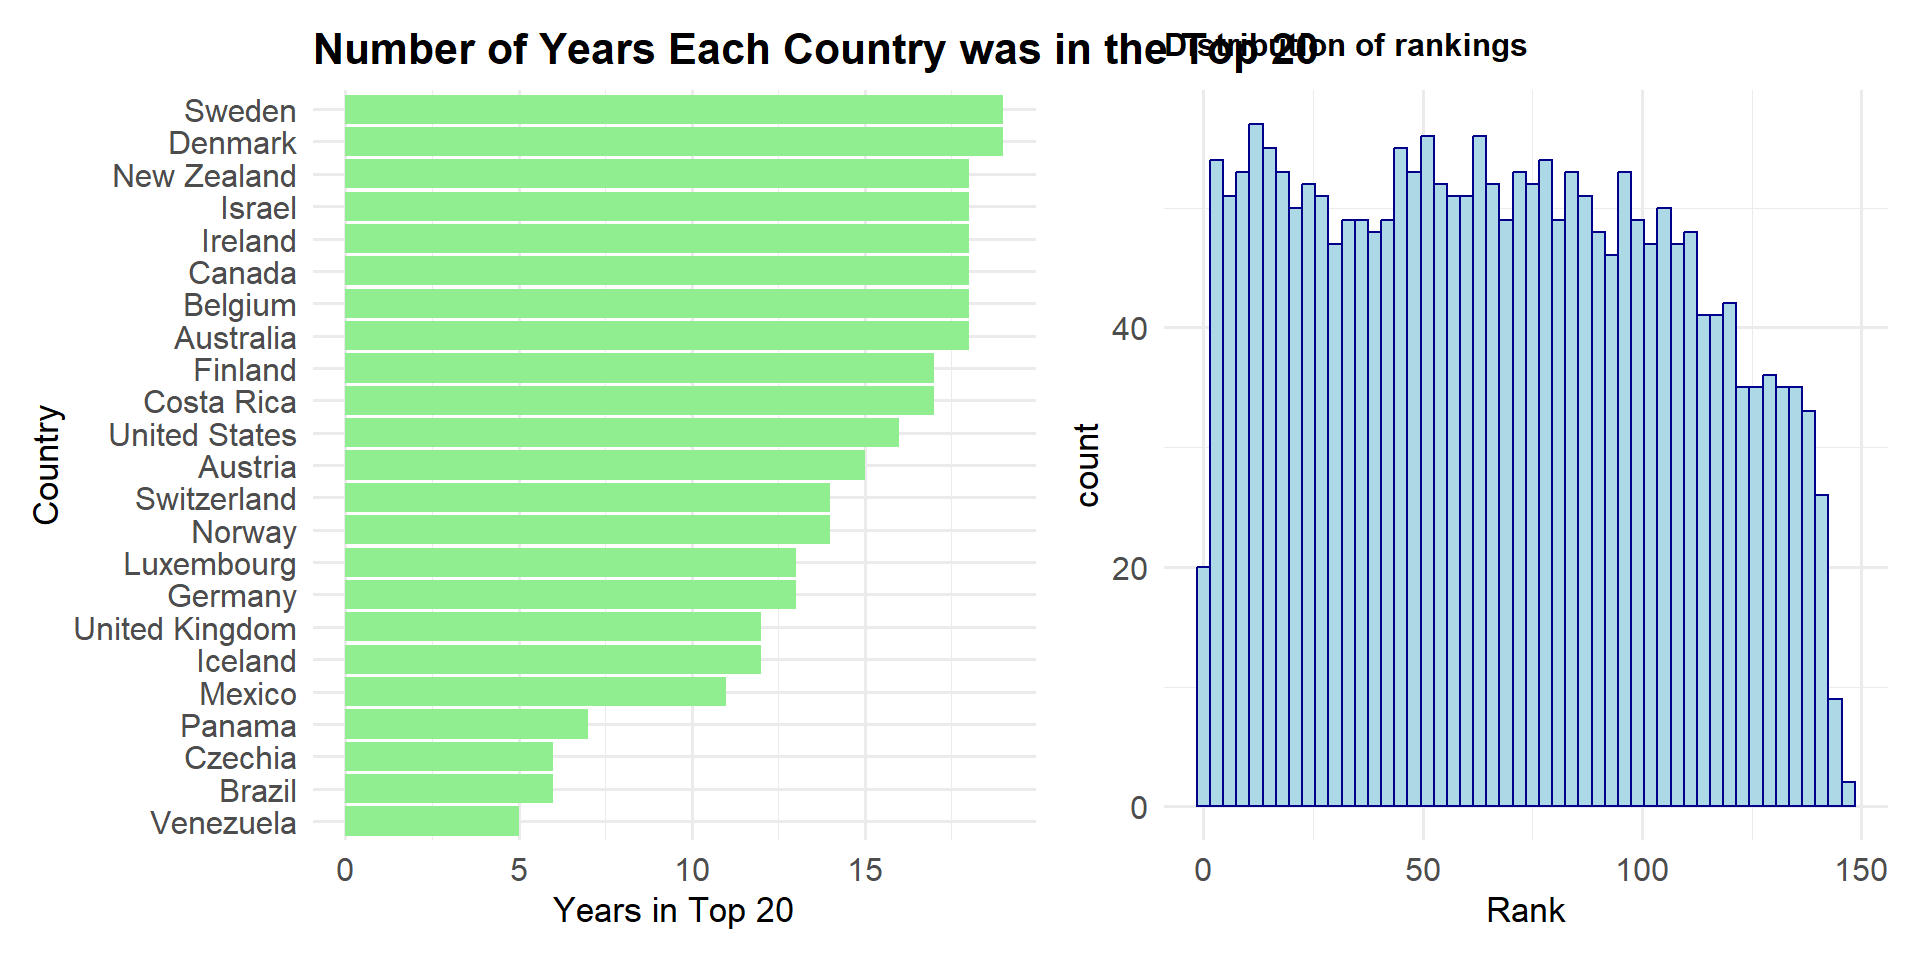
\includegraphics{project_files/figure-latex/top_countries_long-1.pdf}

The distribution of the number of years in the top 20 is kept pretty
limited, only 14 countries have never left the top 20 spot. This goes to
show that being a top country is a perpetual title. Which means there is
merit to asking this question, we think there is a pattern of data that
indicates how consistent a country is at staying at the top of the list.

\#\texttt{\{r\ plot\_Ladder\_score\ ,fig.width=15,\ fig.height=5,\ echo=FALSE,\ warning=FALSE,\ message=FALSE\}\ \#plt1\ \#}

\#This graph's purpose is to show that the columns are good predictors
for the ladder score, and by extension being a top country. This wasn't
unexpected, it's logical that an indicator of a positive trait in a
country's society would impact its overall happiness. And since the
ladder score is what dictates where a country is ranked, it will also
probably take part in the model for our question.

\section{Work Plan}\label{work-plan}

The outcome is the Top-20 column and the predictors currently are all of
the columns. The way we will answer the question is that we will attempt
to find the most contributing variables in order to answer the question.

we will use a variety of methods to answer the question: SHAP
variables,desicion-tree and a logistic regression model, we will attempt
to build those models concurrently and to compare and contrast them.

we would like to receive some conclusive results(the p\_value of some of
the variables will be significant),in all models so after comparison we
could isolate the most relevant factors.

\begin{itemize}
\tightlist
\item
  Data preparation and cleaning. (Bar)
\item
  Exploratory analysis and visualization. (Roni)
\item
  Model building and evaluation. (Roni,Niv)
\item
  Interpretation of results and final reporting. (Amal,Niv)
\end{itemize}

\newpage

Appendix\newline   This Markdown file describes the data structure and
organization for the project.\newline  

we will also elaborate about the pre project data cleaning,\newline  
this data is a addition of WHR(world happiness reports) from 2011 to
2024.\newline   the data cleaning included fixing the country
names(where the standard of naming was changed in between the
reports),erasing countries that dont exist and deleting
duplicates.\newline   we also changed the column names(not all of the
column names were identical in all the reports.)\newline  

Data Columns: \newline  
1. YEAR: the year in which the survey was conducted (the data is from
2011--2024)\newline  
2. Rank -- the country's Rank in the according year (from 1 to 158); not
all countries were ranked plus the rank is by 3 year average.\newline  
3. Country name -- the abbreviated name of the relevant
country.\newline  
4. Ladder score -- the WHR provides a number of the final happiness
score of the current country (from 1.3 to 7.9).\newline  
5. upperwhisker -- the upper boundary of the whisker score (from 1.43 to
7.91).\newline  
6. lowerwhisker -- the lower boundary of the whisker score (from 1.3 to
7.78).\newline  
7. Log GDP per capita -- a normalized version of the country's GDP index
in comparison to the rest of the world (normalized in range from 0 to
2.2).\newline  
8. Social support -- a normalized version of the country's social
support index in comparison to the rest of the world (normalized in
range from 0 to 1.8).\newline  
9. Healthy life expectancy -- a normalized version of the country's
healthy life expectancy index in comparison to the rest of the world
(normalized in range from 0 to 1.13).\newline  
10. Freedom to make life choices -- a normalized version of the
country's freedom to make life choices index in comparison to the rest
of the world (normalized in range from 0 to 1.018).\newline  
11. Generosity -- a normalized version of the country's generosity index
in comparison to the rest of the world (normalized in range from 0 to
0.57).\newline  
12. Perceptions of corruption -- a normalized version of the country's
perceptions of corruption index in comparison to the rest of the world
(normalized in range from 0 to 0.587).\newline  
13. Dystopia + residual -- a normalized version of the country's
dystopia + residual index in comparison to the rest of the world
(normalized in range from -0.11 to 3.482).\newline  
14. Top 20 -- a binary variable indicating whether the country is in the
top 20 in that particular year (the outcome variable).\newline  

Rows: 1,969\newline   Columns: 14\newline   \$ Year 2024, 2023, 2022,
2021, 2020, 2019\ldots{}\newline   \$ Rank 1, 143, 137, 146, 150, 153,
154,\ldots{}\newline   \$ Country\_name ``Finland'', ``Afghanistan'',
``Afghanistan'', \ldots{}\newline   \$ Ladder\_score 7.7360, 1.7210,
1.8590, 2.4040, \ldots{}\newline   \$ upperwhisker 7.810000, 1.775000,
1.923000, 2.\ldots{}\newline   \$ lowerwhisker 7.662000, 1.667000,
1.795000, 2.\ldots{}\newline   \$ Log\_GDP 1.7490000, 0.6280000,
0.6450000,\ldots{}\newline   \$ Social\_support 1.7830000, 0.0000000,
0.0000000,\ldots{}\newline   \$ Life\_expectancy 0.8240000, 0.2420000,
0.0870000,\ldots{}\newline   \$ Freedom\_of\_choices 0.9860000,
0.0000000, 0.0000000,\ldots{}\newline   \$ Generosity 0.1100000,
0.0910000, 0.0930000,\ldots{}\newline   \$ Corruption 0.502000000,
0.088000000, 0.0590\ldots{}\newline \$ Dystopia\_and\_residual 1.782000,
0.672000, 0.976000, 1.\ldots{}\newline   \$ Top\_20 TRUE, FALSE, FALSE,
FALSE, FALSE\ldots{}\newline  

\textbackslash{}\\
\textbf{models and fun} The main model: Decision Tree Like logistic
regression this is also a popular model for classification problems, and
since it can be visualized it is an obvious choice to be one of the
models.

The second model example: Logistic Regression If we're to take a
classification route, then logistic regression would be a good model for
that. We got good results, but again maybe too good. All of the
predictors seem to be strong predictors which was good for the sake of
showing that there is a correlation, but the performance was too
accurate to use as the main model.

\emph{desicion tree models}

we will create 4 diffrent tree models: the first model will be a
decision tree including the Last\_top\_20 parameter and will use the
chronologically split data. the second model will be a decision tree
without the Last\_top\_20 parameter and will use the chronologically
split data. the first model will be a decision tree including the
Last\_top\_20 parameter and will use the randomly split data. the second
model will be a decision tree without the Last\_top\_20 parameter and
will use the randomly split data.

we start with chronologically spliting the data for prior and post 2022
in an almost 80-20 split

\begin{verbatim}
## Train rows: 1542 ( 78.31 % )
\end{verbatim}

\begin{verbatim}
## Test rows : 427 ( 21.69 % )
\end{verbatim}

\begin{verbatim}
##  [1] "Year"                  "Rank"                  "Country_name"         
##  [4] "Ladder_score"          "upperwhisker"          "lowerwhisker"         
##  [7] "Log_GDP"               "Social_support"        "Life_expectancy"      
## [10] "Freedom_of_choices"    "Generosity"            "Corruption"           
## [13] "Dystopia_and_residual" "Top_20"                "Top20_Last"
\end{verbatim}

\emph{first model}

the first model training including top\_20\_last year parameter. looking
the important indicators corruption is the primary indicator of the
tree, despite and the TOP\_20\_last second(showing the importance of
this parameter).
\includegraphics{project_files/figure-latex/unnamed-chunk-3-1.pdf}

\begin{verbatim}
##            Corruption            Top20_Last                  Year 
##             160.14534             122.27920              54.88387 
##       Life_expectancy        Social_support Dystopia_and_residual 
##              47.77010              46.15795              35.16595 
##               Log_GDP    Freedom_of_choices 
##              31.46376              13.49038
\end{verbatim}

the first tree model predictions had a nearly 98\% accuracy which shows
that the model is almost perfect and that the countries that were in the
top 20 are likely to stay there, confirming our primary
assessment,despite the Top\_20\_last not being the primary indicator.

\begin{verbatim}
##          Actual
## Predicted FALSE TRUE
##     FALSE   362    5
##     TRUE      5   55
\end{verbatim}

\begin{verbatim}
## Test Accuracy: 0.9766
\end{verbatim}

\emph{second model} the second model training without the former top\_20
in the second due to the removal of the Top\_20\_last parameter the
corruption takes an even larger part as the primary indicator in the
decision making.

\includegraphics{project_files/figure-latex/unnamed-chunk-5-1.pdf}

\begin{verbatim}
##            Corruption        Social_support       Life_expectancy 
##             190.48757             100.24503              84.74625 
## Dystopia_and_residual               Log_GDP    Freedom_of_choices 
##              73.92820              55.55403              34.89728 
##            Generosity                  Year 
##              27.55772              16.09141
\end{verbatim}

the second model predictions which shows an 82.5\% which is a good
model(not perfect like the first) and shows that even without the
overall scores we are able to predict with reliable accuracy the Top\_20
factor.

\begin{verbatim}
##          Actual
## Predicted FALSE TRUE
##     FALSE   330   38
##     TRUE     37   22
\end{verbatim}

\begin{verbatim}
## Test Accuracy: 0.8244
\end{verbatim}

we will then split the data randomly and check if the results differ.

\emph{third model}

the third model training including top\_20\_last year parameter using
randomized data. in this model unlike the first model(both share the
same parameters) the Top20\_Last and the Year parameters are the primary
indicators by a landslide showing the importance of this factors for the
prediction.

\includegraphics{project_files/figure-latex/unnamed-chunk-8-1.pdf}

\begin{verbatim}
##         Top20_Last               Year         Corruption            Log_GDP 
##         284.927473         165.036219          92.522683          74.454289 
## Freedom_of_choices     Social_support    Life_expectancy         Generosity 
##          55.840717          40.772587           7.509116           6.577438
\end{verbatim}

the third model predictions which shows an 98\% accraucy and knowing how
the model works shows the small movement in the top 20 range on a
randomized data.

\begin{verbatim}
##          Actual
## Predicted FALSE TRUE
##     FALSE   363    8
##     TRUE      4   52
\end{verbatim}

\begin{verbatim}
## Test Accuracy: 0.9719
\end{verbatim}

\emph{fourth model}

the second model training without the former top\_20 with the randomized
data. in this model similarly to the second model corruption is the
primary indicator with a very big margin.

\includegraphics{project_files/figure-latex/unnamed-chunk-10-1.pdf}

\begin{verbatim}
##            Corruption Dystopia_and_residual       Life_expectancy 
##            177.455443             82.534113             36.819540 
##               Log_GDP        Social_support    Freedom_of_choices 
##             33.715976             28.989031              9.824525 
##            Generosity 
##              6.085729
\end{verbatim}

the second model predictions which shows an 95\% which shows that even
despite the removal of the TOP\_20\_last parameter it is still
relatively easy to predict the Top\_20 with a past and future
knowledge(unlike the second model).

\begin{verbatim}
##          Actual
## Predicted FALSE TRUE
##     FALSE   360   18
##     TRUE      7   42
\end{verbatim}

\begin{verbatim}
## Test Accuracy: 0.9415
\end{verbatim}

\emph{logistical regression models}

in this section we created two logistical regression models which differ
in the test and train data they recieve.

\emph{first model} the first model uses a randomly split data and tries
to use logistical regression to determine whether a country is in the
top 20. this model is to successful at 97.5\% accuracy deeming it
ineffective and unreliable.

\begin{verbatim}
## Top_20 ~ Log_GDP + Social_support + Life_expectancy + Freedom_of_choices + 
##     Generosity + Corruption + Dystopia_and_residual
\end{verbatim}

\begin{verbatim}
## Confusion Matrix and Statistics
## 
##           Reference
## Prediction   0   1
##          0 356   5
##          1   5  32
##                                           
##                Accuracy : 0.9749          
##                  95% CI : (0.9543, 0.9879)
##     No Information Rate : 0.907           
##     P-Value [Acc > NIR] : 5.646e-08       
##                                           
##                   Kappa : 0.851           
##                                           
##  Mcnemar's Test P-Value : 1               
##                                           
##             Sensitivity : 0.9861          
##             Specificity : 0.8649          
##          Pos Pred Value : 0.9861          
##          Neg Pred Value : 0.8649          
##              Prevalence : 0.9070          
##          Detection Rate : 0.8945          
##    Detection Prevalence : 0.9070          
##       Balanced Accuracy : 0.9255          
##                                           
##        'Positive' Class : 0               
## 
\end{verbatim}

\emph{second model} the second model uses a timed split data(it uses all
data before 2022 as train data and the rest as test data), and tries to
use logistical regression to determine whether a country is in the top
20. this model as well is to successful at 96\% accuracy deeming it
ineffective and unreliable as well.

\begin{verbatim}
## Confusion Matrix and Statistics
## 
##           Reference
## Prediction   0   1
##          0 361  11
##          1   5  49
##                                           
##                Accuracy : 0.9624          
##                  95% CI : (0.9397, 0.9784)
##     No Information Rate : 0.8592          
##     P-Value [Acc > NIR] : 1.231e-12       
##                                           
##                   Kappa : 0.838           
##                                           
##  Mcnemar's Test P-Value : 0.2113          
##                                           
##             Sensitivity : 0.9863          
##             Specificity : 0.8167          
##          Pos Pred Value : 0.9704          
##          Neg Pred Value : 0.9074          
##              Prevalence : 0.8592          
##          Detection Rate : 0.8474          
##    Detection Prevalence : 0.8732          
##       Balanced Accuracy : 0.9015          
##                                           
##        'Positive' Class : 0               
## 
\end{verbatim}

\end{document}
